\chapter{Определение направлений дальнейших исследований}\label{ch:ch2}

\section{Поиск альтернативных конфигураций каскадов}\label{sec:ch2/sec2}
Дальнейшая работа предполагает подбор с помощью вычислительных экспериментов каскадов, которые могут быть использованы для операции повторного обогащения урана в рамках многократного рецикла. Кандидатами для такого поиска представляются схемы двух следующих типов.

\subsection{Исследование каскадов, использующих дополнительный отбор}\label{sec:ch2/sec1.2}
Схемы, производящие в дополнительном отборе очищенный от минорных четных изотопов полупродукт. Такая композиция с уменьшенным содержанием $^{232, 234, 236}$U, но со схожим с питающей смесью содержанием $^{235}$U, может быть направлена на вход схемы, подобной \ref{fig:Terminal_Dilution}, позволяя добиваться на выходе требуемого содержания по всем изотопам. Однако,  вариации таких схемы, обычно имеют дополнительные потоки питания, как представлено на рисунках \ref{fig:add}

\begin{figure}[ht]
  \begin{minipage}[b][][b]{0.49\linewidth}\centering
    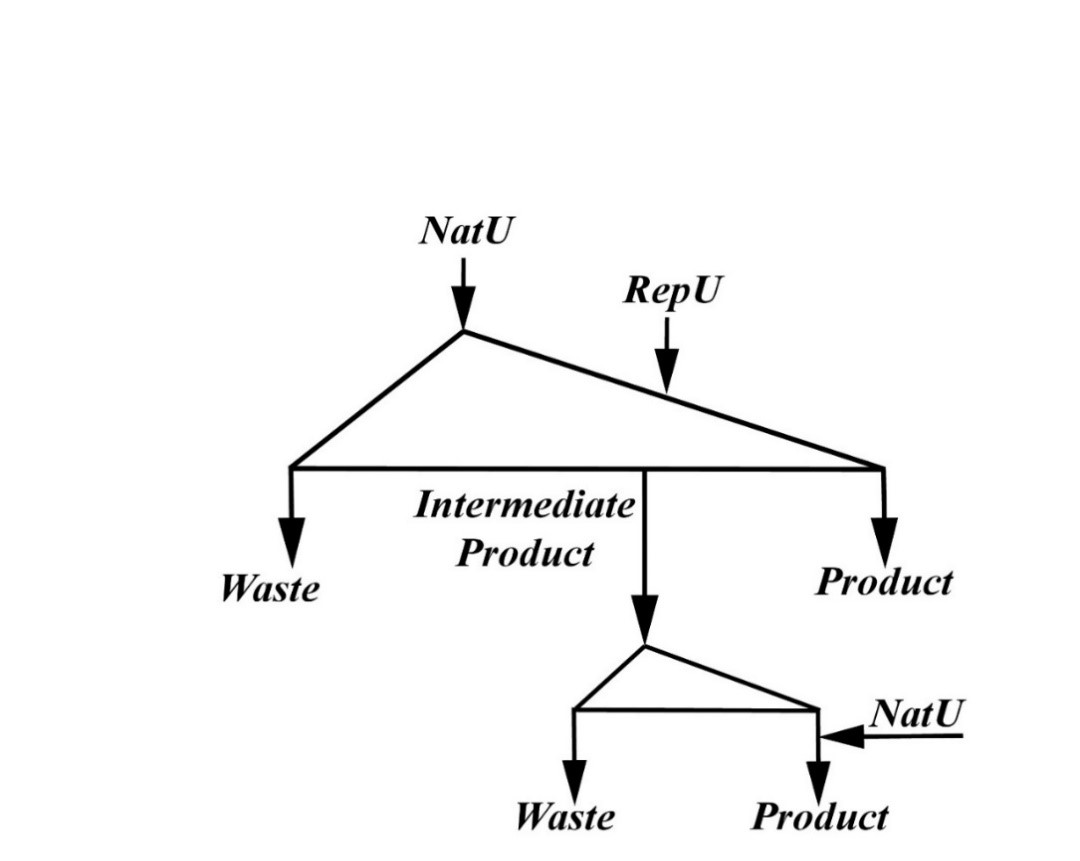
\includegraphics[width=0.9\linewidth]{cascades/add_p} \\ а)
  \end{minipage}
  \hfill
  \begin{minipage}[b][][b]{0.49\linewidth}\centering
    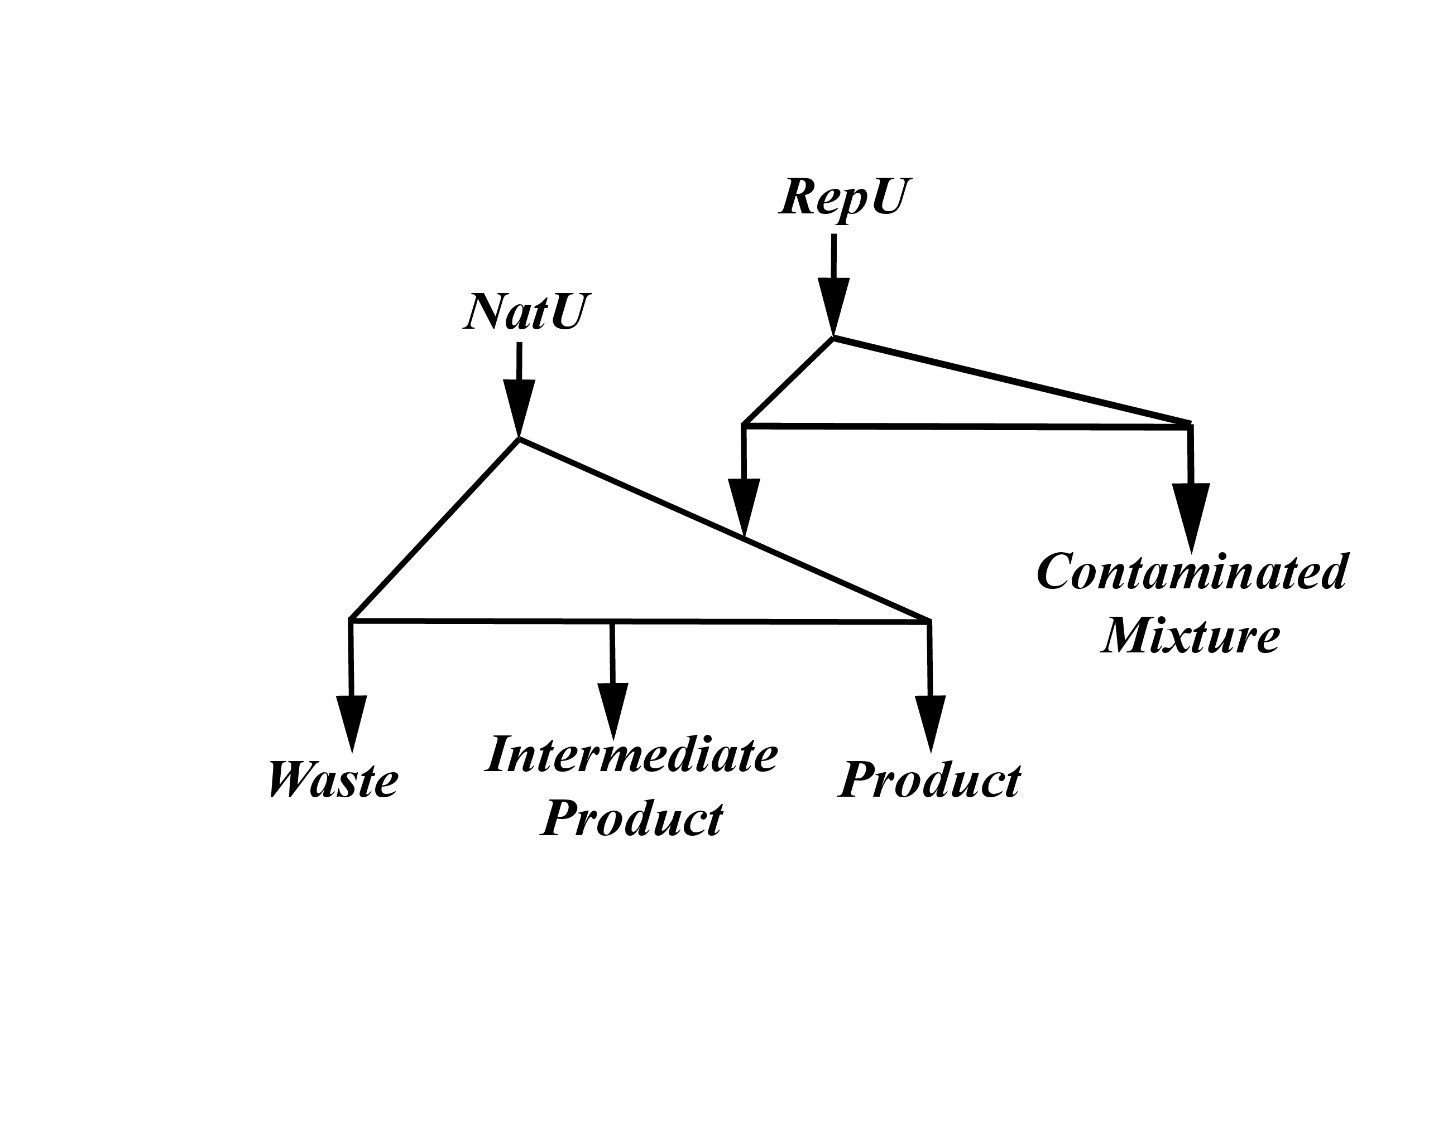
\includegraphics[width=0.9\linewidth]{cascades/add_p2} \\ б)
  \end{minipage}
  \caption{Каскады с дополнительным отбором}
  \label{fig:add}
\end{figure}


\subsection{Исследование каскадов, использующих смещение точки подачи питания}\label{sec:ch2/sec1.1}
С помощью модели квазиидеального каскада необходимо исследование конфигураций, использующих прием в виде варьирования точки подачи питания. Такие схемы тоже требуют анализа на пригодность к приложению в задачах дообогащения регенерированного урана до НОУ, которое может быть использовано в качестве топлива легководных реакторов. Как показано в \cite{palk_2013}, при смещении точки подачи питания каскада относительно оптимума, обеспечивающего минимально возможное число центрифуг, можно существенно изменить концентрацию нецелевых изотопов в отборе и отвале каскада. Такая особенность оптимизации может быть эффективно использована для очистки регенерированного урана от $^{232}$U.

\section{Оптимизация каскадов для полного возврата регенерата}\label{sec:ch2/sec2}
\subsection{Выбор оптимизационных критериев}\label{sec:ch2/sec2.1}

\paragraph{Оценка себестоимости}
Методика оценки в текущих ценах с портала UxC.
\paragraph{Синтетический энергетический показатель}
Сравнение эффективности схем по энергетическому показателю \cite{2019}.
\paragraph{Максимизация вовлечения делящегося изотопа}
Степень извлечения $^{235}$U как ключевой показатель эффективности.
\paragraph{Минимизация соотношения U-232 к U-235 в продукте}

\subsection{Процедура оптимизация каскадов для полного возврата регенерата}\label{sec:ch2/sec2.2}
Выбор схемы для осуществления полного возврата связан с оптимизацией вышеозначенным критериям. Для возможности работы над единой схемой, объединяющей различные варианты обращения с потоком, образующимся на легком конце каскада с индексом 2, предложена схема \ref{fig:Total scheme}. Так как она включает в себя ранее разработанные конфигурации, представленные на рисунках \ref{fig:Tomsk} и \ref{fig:patent}, целесообразно проводить оптимизацию с ее помощью. Полученный результат в этом случае будет сопутствовать оптимальный режим обращения с производимой грязной смесью потока, получаемого на выходе из второго каскда (через \ref{fig:Tomsk} или же через \ref{fig:patent}).
Добавим, что процедура оптимизации может быть выполнена в постановке многокритериальной задачи, а расчетный код может быть оформлен в качестве программного комплекса, выступающего системой поддержки принятия решений.

\begin{figure}[ht]
  \centerfloat{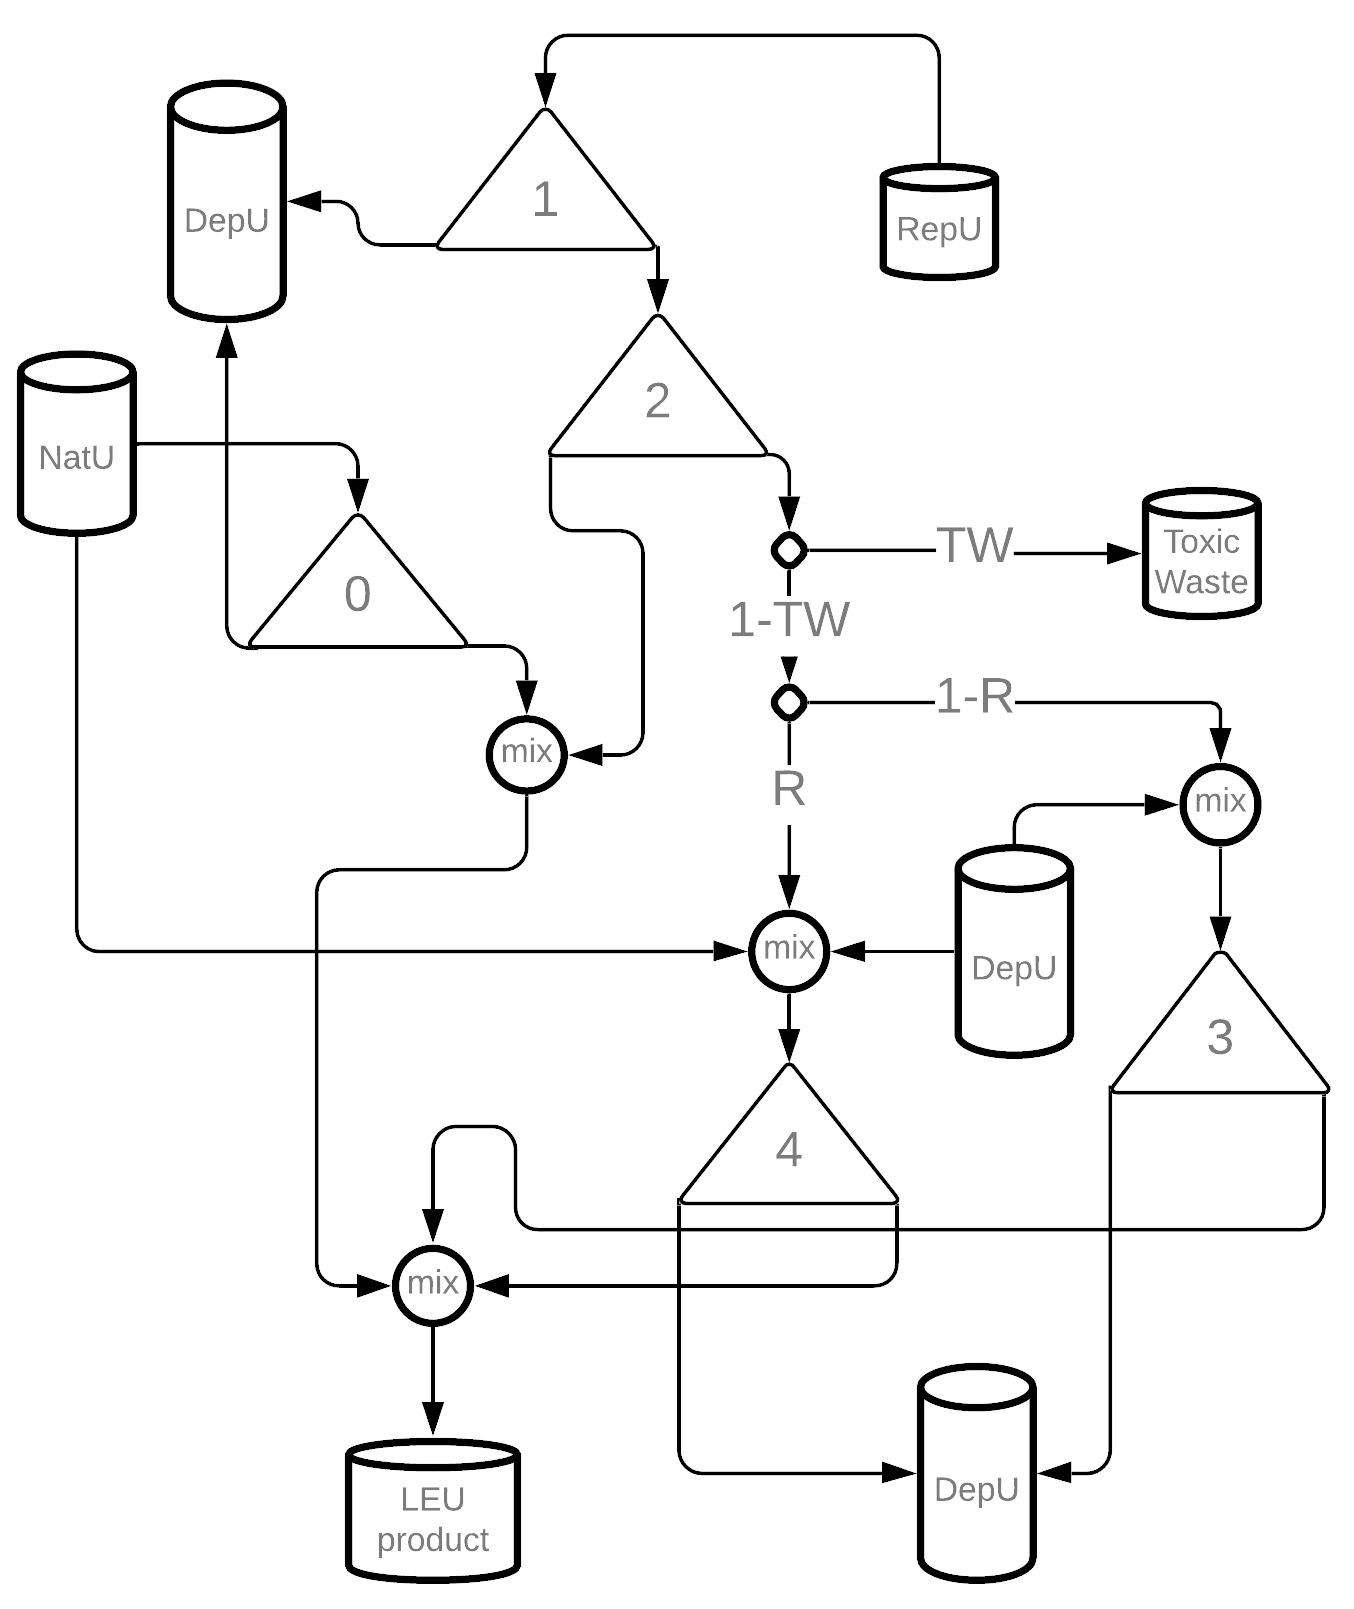
\includegraphics[scale=0.3]{cascades/Total scheme}}
  \caption{Пятикаскадная схема}\label{fig:Total scheme}
\end{figure}

Отметим, что для сравнения схемы с бенчмарком -- ординарным каскадом, необходимо усреднить отвальные концентрации, получаемые в тяжелых фракциях входящих в составную конфигурацию каскадов, и использовать полученное значение концентрации $^{235}$U в отвале ординарного каскада на природном уране, проводя вычисление потребляемых Единиц Работы Разделения (ЕРР).








